\clearpage
\section{Hardware editor}
All computer programs including OghmaNano run on physical computing hardware. There are may combinations of hardware that can be in any computer, some computes have a large number of CPU cores while others only have one. Likewise computers come with differing amounts of memory, hard disk space and GPUs. To help the user get the best out of OghmaNano, there is a hardware editor where the user can configure how OghmaNano behaves on any given computer. This can be accessed through the simulation tab window see Figure \ref{fig:hardware_ribbon}. 

\begin{figure}[H]
\centering
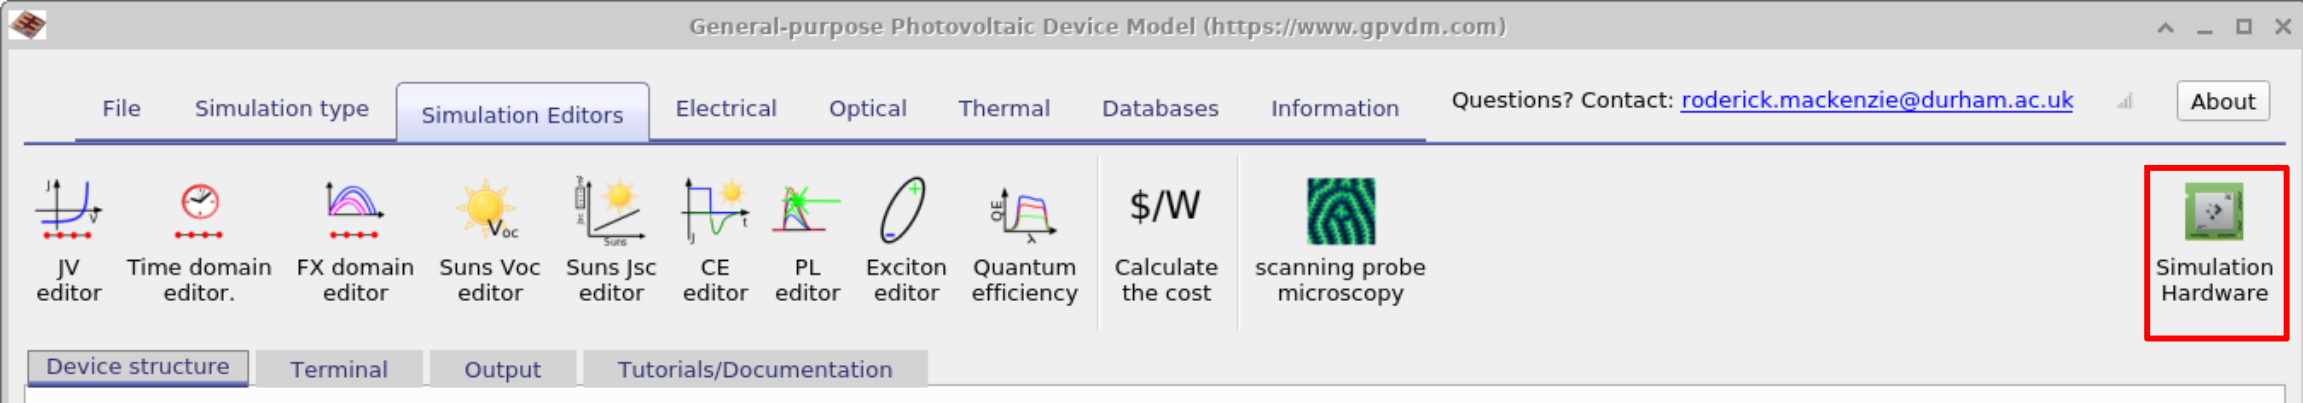
\includegraphics[width=0.9\textwidth,height=0.15\textwidth]{./images/sim_editors/ribbon_hardware.png}
\caption{Opening the hardware editor.}
\label{fig:hardware_ribbon}
\end{figure}

If you click on this it will bring up the hardware editor window which can be seen in Figure \ref{fig:hardware_editor}

\begin{figure}[H]
\centering
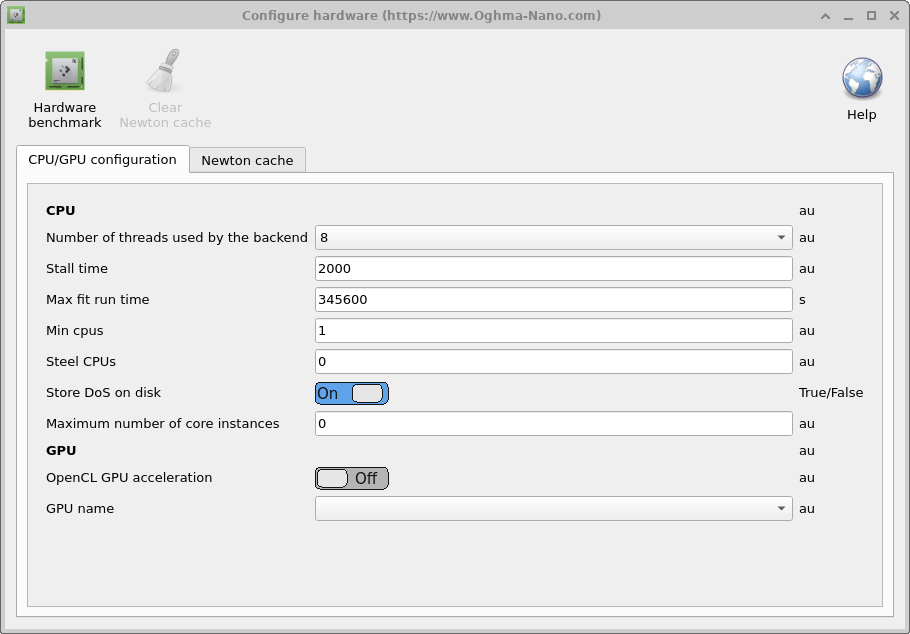
\includegraphics[width=0.7\textwidth,height=0.5\textwidth]{./images/hardware/cpu.png}
\caption{The hardware editor window}
\label{fig:hardware_editor}
\end{figure}

The hardware window is comprised of various tabs which enable the user to edit the configuration and also benchmark your device. 

\subsection{CPU/GPU configuration tab}
This tab is used to configure how OghmaNano interacts with the GPU and CPU it is described in the table below. As described in other parts of this manual in detail there are two parts to OghmaNano there is oghma\_core.exe which is the computational back end and there is oghma\_gui.exe which is the graphical user interface, how both these parts of the model behave can be fine tuned here.

	\begin{itemize}
		\vspace{-0.2cm}\item \emph{Number of threads used by the backend:} This is the maximum number of threads OghmaNano oghma\_core.exe can use. This dictates; the number of simultaneous fits that can be run; the maximum number of optimization simulations that can be run at the same time; the maximum number of threads that are used for FDTD simulations; maximum number of of DoS cache files can generated at the same time; number of frequency domain points that can be run at the same time.
		\vspace{-0.2cm}\item \emph{Maximum number of core instances:} This sets the maximum number of oghma\_core.exe instances that can be started by the GUI. If one is running a parameter scan then this will control the maximum number of simultaneous simulations that can be performed at the same time. If the values of \emph{Number of threads used by the backend} has been set to 4 and one is performing an FDTD simulation, then one sets \emph{Maximum number of core instances} to 8, then the GUI will spawn 8 instances of oghma\_core.exe each using 4 threads, thus 32 CPU cores will be needed.
		\vspace{-0.2cm}\item \emph{Stall time:} Sometimes when running OghmaNano on a supercomputer unattended it can stop running, possibly because of an IO error or network error. This option can be used to set the maximum length of a single simulation. By single simulation I mean a single JV curve, single time domain simulation or single frequency domain simulation, but not a whole fit which will involve running thousands if individual simulations.). So with a value of 2000 seconds the solver will exit, if for example a single JV simulation takes longer than 2000 seconds. In reality any individual simulation should take only a few seconds, so this option acts as a hard backstop if something has gone very wrong. 
		\vspace{-0.2cm}\item \emph{Max fit run time:} This is the maximum time oghma\_core.exe can reside in memory. If any simulation or fit takes longer than this value it will be terminated, again this is a backstop to prevent simulations running forever.  The default value is 4 days. 
		\vspace{-0.2cm}\item \emph{Steel CPUs:} Sometimes when running OghmaNano on a shared PC one will set a simulation running when another user is using a significant number of cores. After a while the other user's simulations will finish running leaving the computer with idling CPUs. If this option is set to \emph{True}, then OghmaNano will monitor the number of free CPUs and if more become available it will use them.
		\vspace{-0.2cm}\item \emph{Min CPUs:} Used with the option above \emph{Steel CPUs} to set the minimum number of CPUs that will be used.
		\vspace{-0.2cm}\item \emph{Store DoS on disk:} OghmaNano stores lookup tables on disk to speed up simulations, if this option is set to false these lookup tables will not be stored.
		\vspace{-0.2cm}\item \emph{OpenCL GPU acceleration:} This enables or disables GPU acceleration, this is used mainly during the FDTD simulations.
		\vspace{-0.2cm}\item \emph{GPU name:} Selects the GPU to use.
	\end{itemize}

\subsection{Newton cache}

When running simulations with a significant number of ODEs, such as 1D devices with a lot of trap states and a lot of spatial points, or when running 2D OFET simulations each voltage step can take a while to compute. This is because the solver must solve each voltage step using Newton's method until it converges. For each each solver step the Jacobian must be built, the matrix inverted multiplied by the residuals and updates to all solver variables calculated. This can take a significant amount of time per step (2000ms). An approach to side step this approach is to store previously calculated answers on disk and then when the user asks the solver to calculated an already calculated problem the answer can be recalled rather than recalculated. This is very useful in OLED design where one is trying to optimise the optical structure of the device but leaves the electrical structure unchanged. One can run new optical simulations with already pre-calcualted electrical solutions.  Configuration options are displayed in the table below.

There is an overhead to using the Newton Cache, so I would only recommend it when solving the electrical problem is very slow indeed. Technically the Newton cache works by taking the MD5 sum of the Fermi-levels and the potentials to generate a hash of the electrical problem. This is then compared to what exists on disk. If a precalculated answer is found, the Fermi-levels/potentials are updated to the values found on disk. The cache is stored in oghma\_local\\cache, each pre solvedsolution is stored as a new binary file. Each simulation run generates an index file where all MD5 sums from that simulation are stored. Once the cache becomes full OghmaNano deletes simulation results in batches based on the index files.

\begin{figure}[H]
\centering
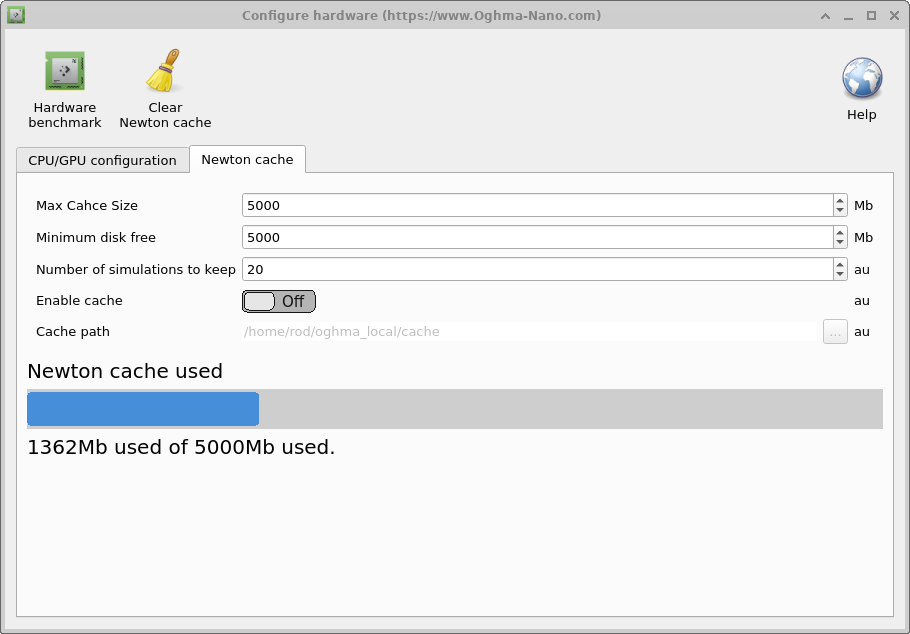
\includegraphics[width=0.7\textwidth,height=0.5\textwidth]{./images/hardware/newton.png}
\caption{The Newton cache editor}
\label{fig:newton_cache_editor}
\end{figure}


	\begin{itemize}
		\vspace{-0.2cm}\item \emph{Maximum cache size:} Sets the maximum size of the cache in Mb. I would recommend around 1Gb.
		\vspace{-0.2cm}\item \emph{Minimum disk free:} Sets the minimum amount of disk space needed to use the cache, this option is designe dto prevent the cache filling the disk I would set it to around 5Gb.
 		\vspace{-0.2cm}\item \emph{Number of simulations to keep:} This will set the maximum number of simulation runs to keep, I would set it to between 20 and 100.
 		\vspace{-0.2cm}\item \emph{Enable cache:} This enables or disables the Newton Cache, the default and recommended option is False.
	\end{itemize}

\subsection{Hardware benchmark}
In the top left of hardware window \ref{fig:newton_cache_editor} there is a button called \emph{Hardware benchmark}. If this is clicked then OghmaNano will benchmark your hardware, the result of such a benchmark can be seen in \ref{fig:hardware_benchmark}. This runs benchmarks your CPUs ability to calculate \emph{sin},\emph{exp} and allocate/deallocate memory in blocks. It displays how long it took to do a few thousand operations as well as an \emph{R} (aka Roderick) value. This is defined as R=\emph{Time taken to do the calculation on your PC}/\emph{The time take to do the calculation on my PC}. Thus smaller values mean your PC is faster than mine. My PC is a Intel(R) Core(TM) i7-4900MQ CPU @ 2.80GHz in a 2017 Lenovo thinkpad. So most modern computers should be faster. If you have good CPU performance but your simulations are running slower than my YouTube videos then this is invariably due to bad IO speed, caused by virus killers, storing the simulations on OneDrive, using networked drives, using slow USB storage etc.

\begin{figure}[H]
\centering
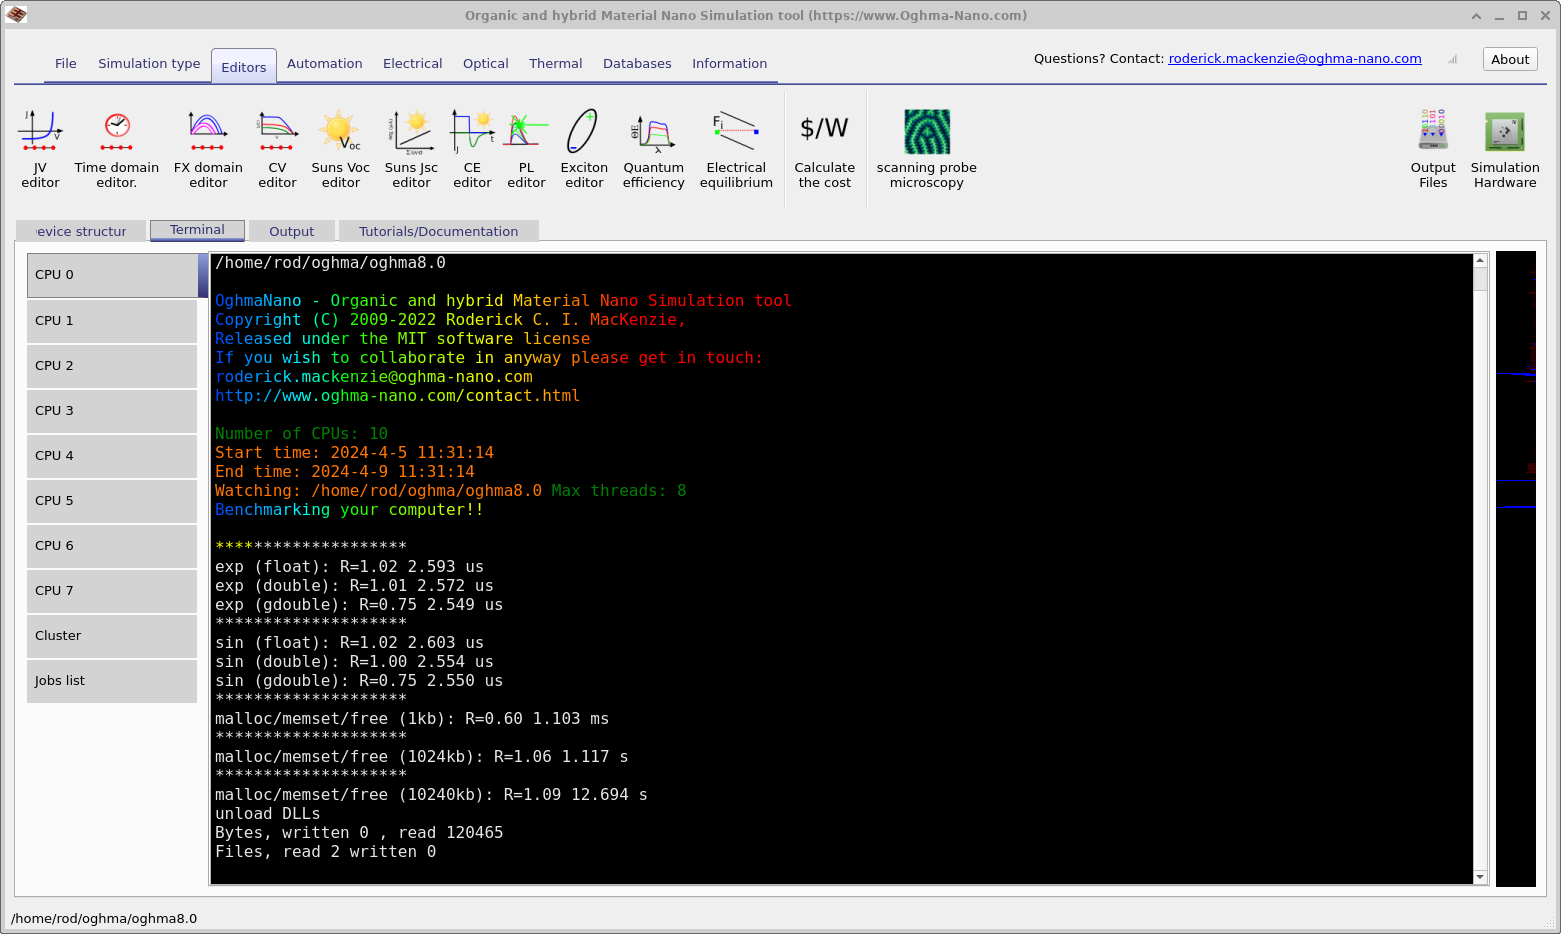
\includegraphics[width=1.0\textwidth,height=0.8\textwidth]{./images/hardware/benchmark.png}
\caption{Running a hardware benchmark}
\label{fig:hardware_benchmark}
\end{figure}

